Die entwickelten Methoden haben gezeigt, dass es möglich ist, einerseits den \textit{NAO} Roboter eigenständig Spielelogiken und Spielfeld und -standerkennung durchführen, andererseits die daraus resultierenden Spielzüge auch selbst ausführen zu lassen. Sowohl das Spielen von \textit{TicTacToe} als auch \textit{Vier gewinnt} sind keine neuen Ideen, beide wurden schon mehrfach und in verschiedener Ausführung für die Roboter implementiert\cite{nao_tictactoe_magnets, nao_tictactoe_pen, nao_connect4_1, nao_connect4_2}. Die hier aufgeführten Ansätze basieren jedoch einerseits auf dem Szenario \textit{NAO vs. Mensch}, andererseits benötigen sie auch immer Hilfsmittel wie Stifte oder Spielsteine, um den Spielzug zu tätigen. Der hier entwickelte Ansatz verzichtet auf all das, indem es durch das jederzeit verfügbare Material Aluminiumfolie die Roboter dazu befähigt, eigenständig Klicks auf einem Touchpad zu tätigen. Zudem läuft das entwickelte Python-Skript des Projektes auf dem Roboter selbst und kann auf Wunsch direkt beim Start des \textit{NAO} ausgeführt werden, wobei die Kalibration des Roboters zum Tablet hin jedoch entscheidend für das Spielen ist und vorher ausgeführt werden sollte. Dies lässt sich bei Bedarf vor das eigentliche \dq Hauptmenü\dq schalten.  

Ein im Rahmen des Projektes nicht mehr zu realisierendes Feature war das jederzeit mögliche Abbrechen des Spiels durch Knopfdruck. Hierzu müsste jedoch nebenläufig programmiert werden, welches sich im verbliebenen Zeitrahmen und den Einschränkungen durch die Python-Version als schwierig erwiesen hat.

Problematisch haben sich bei der Arbeit einerseits die veraltete Python-Version ($2.7.18$ vs. Stand September 2023 $3.11.5$), andererseits viele mechanische Probleme mit den Robotern. Von sechs vorhandenen \textit{NAOs} waren nur zwei in der Lage, den rechten Arm korrekt zu bewegen. Somit blieben nur zwei Roboter für das Probjekt übrig, einen mit Version $5$ (naoqi Version $2.1.4$, IP: $10.30.4.13$), und einen mit Version $6$ (naoqi Version $2.8.6$, IP: $10.30.4.31$).

Beim dem Roboter mit der neueren naoqi Version (2.8.6) gab es außerdem ein weiteres Problem. Wie sich zeigte stellte der Roboter seinen rechten Arm oft falsch ein, obwohl die übermittelten Werte korrekt waren. In der Abbildung unten sieht man die Differenz zwischen den übergebenen Werten des linken und rechten Arms und den Werten, die tatsächlich von der Sensorik des Roboters erfasst wurden. 
\begin{figure}[!htbp]
    \centering
    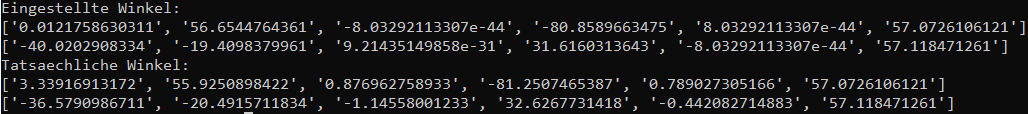
\includegraphics[width=1\linewidth]{bilder/bilder_movement/WinkelDifferenz.PNG}
\end{figure}
Dabei fällt bei dem Motor ShoulderPitch des rechten Arms auf, dass die Einstellung 40 Grad beträgt, aber der Nao seinen Arm nur 36 Grad nach oben bewegt. Dieser Fehler tritt bei dem besagten Roboter immer wieder auf. Diese Einstellung ist wichtig, um das Tablet zum Roboter korrekt aufzustellen. Ähnliche Ungenauigkeiten treten auch bei den anderen Nao Robotern auf sind hier jedoch nicht so gravierend, wodurch dies nur zu weniger präzisen Klicks führt. 
